%%%%%%%%%%%%%%
%% Run LaTeX on this file several times to get Table of Contents,
%% cross-references, and citations.

%% If you have font problems, you may edit the w-bookps.sty file
%% to customize the font names to match those on your system.

%% w-bksamp.tex. Current Version: Feb 16, 2012
%%%%%%%%%%%%%%%%%%%%%%%%%%%%%%%%%%%%%%%%%%%%%%%%%%%%%%%%%%%%%%%%
%
%  Sample file for
%  Wiley Book Style, Design No.: SD 001B, 7x10
%  Wiley Book Style, Design No.: SD 004B, 6x9
%
%
%  Prepared by Amy Hendrickson, TeXnology Inc.
%  http://www.texnology.com
%%%%%%%%%%%%%%%%%%%%%%%%%%%%%%%%%%%%%%%%%%%%%%%%%%%%%%%%%%%%%%%%

%%%%%%%%%%%%%
% 7x10
%\documentclass{wileySev}

% 6x9
\documentclass{wileySix}

\usepackage{graphicx}
\usepackage{listings}
\usepackage{float}
\usepackage[urlcolor=blue, colorlinks=true]{hyperref}
\usepackage{color}

\definecolor{codegreen}{rgb}{0,0.6,0}
\definecolor{codegray}{rgb}{0.5,0.5,0.5}
\definecolor{codepurple}{rgb}{0.58,0,0.82}
\definecolor{backcolour}{rgb}{0.95,0.95,0.92}

\lstdefinestyle{mystyle}{
    backgroundcolor=\color{backcolour},
    commentstyle=\color{codegreen},
    keywordstyle=\color{magenta},
    numberstyle=\tiny\color{codegray},
    stringstyle=\color{codepurple},
    basicstyle=\footnotesize,
    breakatwhitespace=false,
    breaklines=true,
    captionpos=b,
    keepspaces=true,
    numbers=left,
    numbersep=5pt,
    showspaces=false,
    showstringspaces=false,
    showtabs=false,
    tabsize=2,
    language=sh
}

\lstset{style=mystyle}

%%%%%%%
%% for times math: However, this package disables bold math (!)
%% \mathbf{x} will still work, but you will not have bold math
%% in section heads or chapter titles. If you don't use math
%% in those environments, mathptmx might be a good choice.

% \usepackage{mathptmx}

% For PostScript text
\usepackage{w-bookps}

%%%%%%%%%%%%%%%%%%%%%%%%%%%%%%%%%%%%%%%%%%%%%%%%%%%%%%%%%%%%%%%%
%% Other packages you might want to use:

% for chapter bibliography made with BibTeX
% \usepackage{chapterbib}

% for multiple indices
% \usepackage{multind}

% for answers to problems
% \usepackage{answers}

%%%%%%%%%%%%%%%%%%%%%%%%%%%%%%
%% Change options here if you want:
%%
%% How many levels of section head would you like numbered?
%% 0= no section numbers, 1= section, 2= subsection, 3= subsubsection
%%==>>
\setcounter{secnumdepth}{3}

%% How many levels of section head would you like to appear in the
%% Table of Contents?
%% 0= chapter titles, 1= section titles, 2= subsection titles,
%% 3= subsubsection titles.
%%==>>
\setcounter{tocdepth}{2}

%% Cropmarks? good for final page makeup
%% \docropmarks

%%%%%%%%%%%%%%%%%%%%%%%%%%%%%%
%
% DRAFT
%
% Uncomment to get double spacing between lines, current date and time
% printed at bottom of page.
% \draft
% (If you want to keep tables from becoming double spaced also uncomment
% this):
% \renewcommand{\arraystretch}{0.6}
%%%%%%%%%%%%%%%%%%%%%%%%%%%%%%

%%%%%%% Demo of section head containing sample macro:
%% To get a macro to expand correctly in a section head, with upper and
%% lower case math, put the definition and set the box
%% before \begin{document}, so that when it appears in the
%% table of contents it will also work:

\newcommand{\VT}[1]{\ensuremath{{V_{T#1}}}}

%% use a box to expand the macro before we put it into the section head:

\newbox\sectsavebox
\setbox\sectsavebox=\hbox{\boldmath\VT{xyz}}

%%%%%%%%%%%%%%%%% End Demo


\begin{document}


\booktitle{SIG (Sistem Informasi Geografis)}
\subtitle{Semester 5}

\authors{D4TI3A\\
\affil{Angkatan 2017}
%Floyd J. Fowler, Jr.\\
%\affil{University of New Mexico}
}

\offprintinfo{SIG (Sistem Informasi Geografis), First Edition}{D4TI3A}

%% Can use \\ if title, and edition are too wide, ie,
%% \offprintinfo{Survey Methodology,\\ Second Edition}{Robert M. Groves}

%%%%%%%%%%%%%%%%%%%%%%%%%%%%%%
%%
\halftitlepage

%\titlepage


\begin{copyrightpage}{2019}
\input{info/copyrightpage}
\end{copyrightpage}

\dedication{`Jika Kamu tidak dapat menahan lelahnya belajar,
Maka kamu harus sanggup menahan perihnya Kebodohan.'
~Imam Syafi'i~}

\begin{contributors}
\input{info/contributors}
\end{contributors}

\contentsinbrief
\tableofcontents
\listoffigures
\listoftables
\lstlistoflistings


\begin{foreword}
\input{info/foreword}
\end{foreword}

\begin{preface}
\input{info/preface}
\end{preface}


\begin{acknowledgments}
\input{info/acknowledgments}
\end{acknowledgments}

\begin{acronyms}
\input{info/acronyms}
\end{acronyms}

\begin{glossary}
\input{info/glossary}
\end{glossary}

\begin{symbols}
\input{info/symbols}
\end{symbols}

\begin{introduction}
\input{info/introduction}
\end{introduction}

%%%%%%%%%%%%%%%%%% Isi Buku %%%%%%%%%%%%%%%%%%
\chapter{Tugas Pertama}
\input{chapters/tugas1/1174xxx}
\input{chapters/tugas1/1174027}
\input{chapters/tugas1/1174026}
\input{chapters/tugas1/1174012}
\input{chapters/tugas1/1174009}
\section{SRI RAHAYU (1174015)}
\subsection{Pengertian SIG}
Geografi adalah ilmu yang mempelajari tentang lokasi serta persamaan dan perbedaan variasi keruangan atas fenomena fisik, dan manusia di atas permukaan bumi. Kata geografi berasal dari Bahasa Yunani yaitu gêo "Bumi", dan graphein "tulisan" atau "menjelaskan". Para sarjana, praktisi, atau penulis di bidang geografi disebut geograf atau geografer.Geografi juga merupakan nama judul buku bersejarah pada subjek ini, yang terkenal adalah Geographia tulisan Klaudios Ptolemaios pada abad kedua.Geografi lebih dari sekadar kartografi, studi tentang peta. Geografi tidak hanya menjawab apa, dan di mana di atas muka bumi, tapi juga mengapa di situ, dan tidak di tempat lainnya, kadang diartikan dengan "lokasi pada ruang." Geografi mempelajari hal ini, baik yang disebabkan oleh alam atau manusia. Juga mempelajari akibat yang disebabkan dari perbedaan yang terjadi itu.
Sistem informasi geografis (SIG) adalah sistem yang didesain untuk menangkap, menyimpan, mengolah, menganalisa, serta mempresentasikan data spasial.Dengan menghubungkan berbagai jenis data yang awalnya dianggap tidak berhubungan, SIG dapat membantu manusia dalam berbagai aspek pekerjaan. Proses menghubungkan ini umumnya dilakukan dalam konteks lokasi (spasial) dan waktu (temporal) yang sama.

\subsection{Sejarah SIG}
Pada awalnya, peta hanya memiliki satu atau dua informasi saja didalamnya, sehingga jika seorang analis ingin mendapatkan informasi tambahan, dia harus melakukan overlay.Salah satu proses overlay pertama yang juga dianggap sebagai penggunaan analisa spasial pertama secara sukses adalah oleh John Snow di London pada tahun 1854. Dia melakukan pemetaan terhadap lokasi orang-orang yang mengidap penyakit cholera dan menghubungkannya dengan peta penyediaan air minum London.Pada awal abad ke-20, penggunaan teknik photozincography mulai meluas. Teknik ini memungkinkan peta terdiri dari beberapa layer yang nantinnya dapat diubah secara mandiri dari layer lainnya. Hal ini berguna untuk melakukan overlay dan analisa peta sesuai dengan layer yang dibutuhkan.Pada teknik ini, layer-layer yang ada dibuat dari film plastik atau lapisan kertas kalkir sehingga dapat digabungkan menjadi satu peta besar. Namun, teknik ini belum dapat dianggap sebagai SIG karena tidak terdapat database yang menghubungkan peta-peta tersebut.Pada tahun 1960, Canada mengembangkan sistem SIG pertamanya yang disebut CGIS atau Canada Geographic Information System. Sistem ini digunakan untuk menyimpan, mengolah, dan menganalisa informasi yang dimiliki oleh badan pertanahan Canada.
Data Yang Digunakan dalam Sistem Informasi Geografis
Terdapat dua jenis data yang umumnya digunakan dalam SIG, yaitu data spasial dan data aspasial.
\begin{itemize}
	\item Data Spasial
	Data spasial adalah data yang memiliki informasi lokasi pada data tersebut. Informasi lokasi ini umumnya berbentuk sistem koordinat baik itu koordinat geografis ataupun koordinat proyeksi.
Data spasial umumnya digunakan untuk menunjukkan lokasi dari suatu obyek/kenampakan pada dunia nyata.Terdapat dua jenis data spasial yaitu vektor dan raster. Kedua jenis data ini memiliki perbedaan sifat dan kegunaannya. Oleh karena itu, penggunaannya sangat tergantung dengan kondisi dan hasil yang ingin dicapai.

	\item Data Vektor
	Data vektor adalah data yang direpresentasikan dengan garis, titik, atau polygon. Data vektor dihasilkan dari digitasi data raster ataupun penggambaran langsung obyek dunia nyata pada peta. Oleh karena itu, data vektor lebih sulit dibuat dibandingkan dengan data raster.
	
\end{itemize}
\subsection{Koordinat SIG}
Koordinat adalah suatu titik yang didapatkan dari hasil perpotongan dari garis latitude (lintang) dengan garis bujur (longitude) sehingga akan menunjukan lokasi pada suatu daerah. Umumnya koordinat dibedakan menjadi koordinat Geographic dan Universal Transver Mercator (UTM). 

Contoh data aspasial adalah data atribut suatu obyek. Misal pada suatu peta terdapat titik berwarna hitam pada koordinat tertentu, kita tidak akan tahu titik tersebut bermakna apa tanpa adanya penjelas yaitu legenda. Legenda adalah salah satu contoh data aspasial.
Sistem informasi geografis modern menggunakan data digital untuk proses analisa dan Y666penafsirannya. Berikut ini adalah beberapa metode pengumpulan data untuk analisa SIG.
Digitasi adalah proses mendigitalkan data yang bersifat fisik. Hal ini perlu dilakukan karena mayoritas data perpetaan masih berada dalam bentuk fisik seperti pada lembaran film atau kertas peta.
Proses ini dapat dilakukan dengan cara memasukkan data fisik seperti foto dan peta kedalam mesin, atau men-scan data tersebut dan mendigitasinya secara manual dengan aplikasi.Proses digitasi akan mengubah data raster menjadi data vektor yang dapat diolah dan dianalisa oleh aplikasi SIG.
Survey juga merupakan bagian yang sangat penting dari SIG. Survey meliputi aktivitas pengambilan data langsung di tempatSurvey menghasilkan data yang nantinya dapat langsung dimasukkan kedalam basis data SIG dengan menggunakan coordinate geometry (COGO).Meskipun telah ada teknologi penginderaan jauh, survey masih sangat dibutuhkan dalam proses pemetaan. Hal ini disebabkan oleh keberadaan informasi-informasi detail lokasi yang mungkin tidak dapat ditangkap dan digambarkan oleh penginderaan jauh.
 
Penginderaan Jauh
Penginderaan jauh adalah metode pengambilan informasi dan pencatatan rupabumi suatu wilayah dengan menggunakan wahana tertentu.Sesuai dengan namanya, surveyor yang menggunakan penginderaan jauh umumnya berlokasi jauh atau tidak langsung berada di wilayah survey. Hal ini dapat terjadi karena kemajuan teknologi pada bidang foto udara, sensor, pesawat, serta satelit.Penginderaan jauh umumnya dilakukan dengan menggunakan foto udara dari pesawat, foto satelit, atau teknologi drone.

\subsection{Data Geospasial SIG}
GPS atau Global Positioning System adalah sistem penentuan lokasi global yang memanfaatkan satelit untuk melakukan triangulasi lokasi perangkat.
Global positioning system berkerja dengan cara menerima sinyal dari satelit yang nantinya akan digunakan untuk melakukan triangulasi lokasi. Oleh karena itu, GPS hanya dapat berfungsi secara akurat jika terdapat 3 atau lebih satelit yang mengirimkan sinyal.
Selain itu, GPS juga harus memiliki koneksi sinyal yang bagus dengan satelit tersebut agar dapat memprediksi lokasi secara akurat.Sekarang, GPS sudah memiliki akurasi dibawah 10m sehingga mengurangi galat saat melakukan perhitungan atau navigasi. GPS navigais tertentu bahkan sudah mencapai akurasi dibawah 3-5m, sedangkan GPS untuk survei dan pemetaan sudah memiliki akurasi dalam rentang milimeter.Meskipun begitu, perangkat GPS yang memiliki kualitas dan akurasi tinggi sangat sulit didapatkan dan memiliki harga yang mahal. Oleh karena itu, tidak semua orang dapat mengakses sebuah GPS.
SIG dapat digunakan untuk melakukan analisa tutupan lahan dengan menginterpretasikan foto udara atau citra satelit.Dengan adanya informasi mengenai tutupan lahan, pihak pemerintah dan perencana wilayah dapat dengan lebih mudah memantau tutupan lahan serta kesesuaiannya dengan zonasi.Analisa TopografiKetinggian dan pola ketinggian suatu wilayah dapat diketahui dan dianalisa dengan menggunakan sistem informasi geografis.Sumber data yang diperlukan untuk analisa ini adalah citra satelit yang memiliki informasi ketinggian. Untuk analisa topografi, sangat sulit menggunakan foto udara konvensional karena sulit mengetahui ketinggian suatu tempat dari sebuah foto.Output yang dihasilkan dari analisa topografi adalah peta DEM (Digital elevation model) serta peta topografi suatu wilayah.Analisa topografi sangat penting dilakukan karena sering digunakan sebagai dasar dari pembuatan peta-peta lainnya.Analisa HidrologiSeorang ahli SIG dapat melakukan analisa dan modelling pergerakan air atau sistem hidrologi pada suatu wilayah dengan menggunakan sistem informasi geografis.Informasi aliran air, debit air, serta kualitas air dapat dipadukan dengan informasi ketinggian, kelerengan, serta morfologi sehingga menciptakan peta aliran air yang lebih komprehensif dan akurat

\subsection{Link}
\href{https://youtu.be/T2lvY-cI0IA}{}
\subsection{Plagiarism}
\begin{figure}[H]
	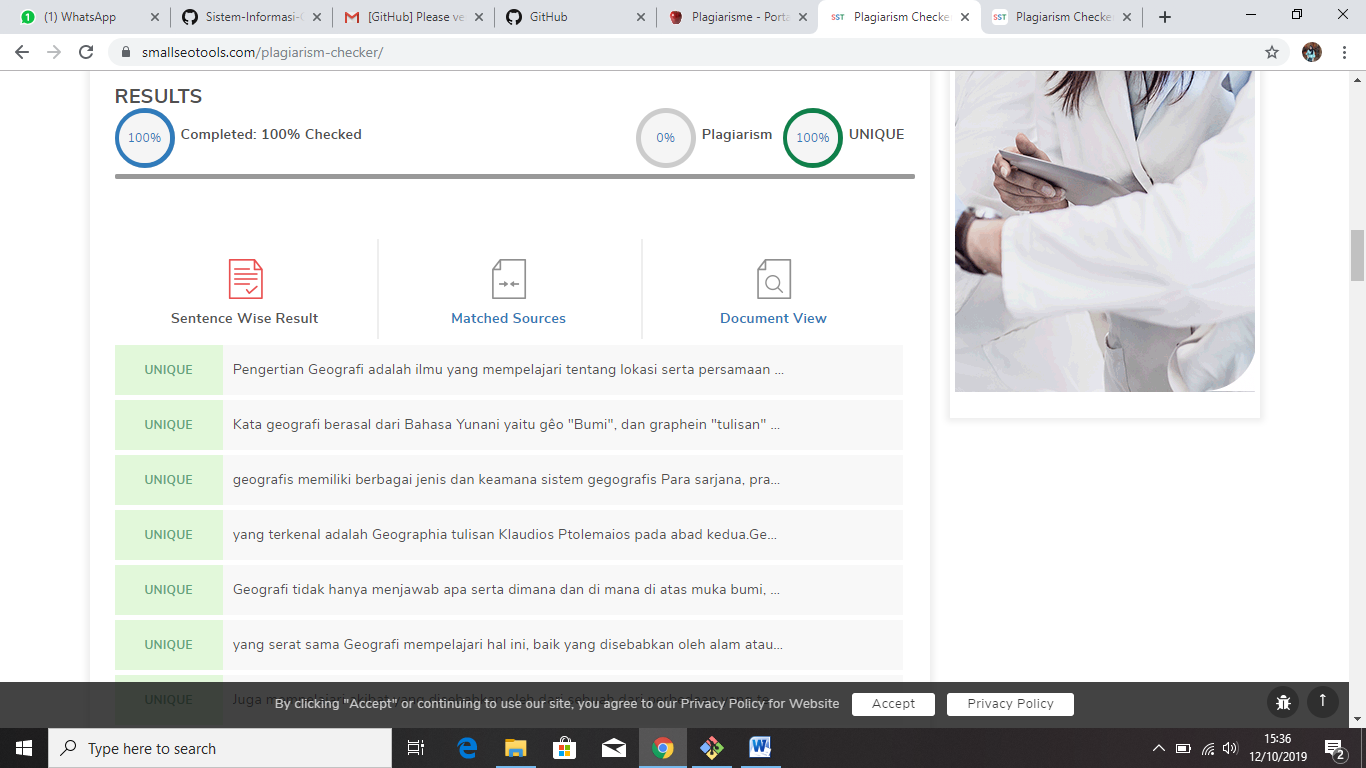
\includegraphics[width=4cm]{figures/1174015/plagiat.png}
	\centering
	\caption{plagiat.}
\end{figure}

\subsection{Cara Penggunaan}
\subsubsection{Gambar}

\hfill\break

Contoh Gambar
\begin{figure}[H]
	\includegraphics[width=4cm]{figures/himatif.png}
	\centering
	\caption{Contoh gambar.}
\end{figure}

\subsubsection{List}
\begin{enumerate}
	\item Satu
	\item Dua
\end{enumerate}

\begin{itemize}
	\item Satu
	\item Dua
\end{itemize}

\href{link kamu}{alias}
contoh link
\href{https://www.google.com/}{klik me}
%\chapter{Tugas Kedua}
%\input{chapters/tugas2/1174xxx}
\bibliographystyle{IEEEtran}
%\def\bibfont{\normalsize}
\bibliography{references}
%%%%%%%%%%%%%%%%%%%%%%%%%%%%%%%%%%%%%%%%%%%%%%


%%%%%%%%%%%%%%%
%%  The default LaTeX Index
%%  Don't need to add any commands before \begin{document}
\printindex

%%%% Making an index
%%
%% 1. Make index entries, don't leave any spaces so that they
%% will be sorted correctly.
%%
%% \index{term}
%% \index{term!subterm}
%% \index{term!subterm!subsubterm}
%%
%% 2. Run LaTeX several times to produce <filename>.idx
%%
%% 3. On command line, type  makeindx <filename> which
%% will produce <filename>.ind
%%
%% 4. Type \printindex to make the index appear in your book.
%%
%% 5. If you would like to edit <filename>.ind
%% you may do so. See docs.pdf for more information.
%%
%%%%%%%%%%%%%%%%%%%%%%%%%%%%%%

%%%%%%%%%%%%%% Making Multiple Indices %%%%%%%%%%%%%%%%
%% 1.
%% \usepackage{multind}
%% \makeindex{book}
%% \makeindex{authors}
%% \begin{document}
%%
%% 2.
%% % add index terms to your book, ie,
%% \index{book}{A term to go to the topic index}
%% \index{authors}{Put this author in the author index}
%%
%% \index{book}{Cows}
%% \index{book}{Cows!Jersey}
%% \index{book}{Cows!Jersey!Brown}
%%
%% \index{author}{Douglas Adams}
%% \index{author}{Boethius}
%% \index{author}{Mark Twain}
%%
%% 3. On command line type
%% makeindex topic
%% makeindex authors
%%
%% 4.
%% this is a Wiley command to make the indices print:
%% \multiprintindex{book}{Topic index}
%% \multiprintindex{authors}{Author index}

\end{document}

